\documentclass{beamer}
\usepackage[utf8]{inputenc}

\usetheme{Boadilla}
\usecolortheme{lily}
\usepackage{amsmath,amssymb,amsfonts,amsthm}
\usepackage{mathtools}
\usepackage{txfonts}
\usepackage{tkz-euclide}
\usepackage{listings}
\usepackage{multicol}
\usepackage{adjustbox}
\usepackage{array}
\usepackage{tabularx}
\usepackage{lmodern}
\usepackage{gvv}
\usepackage{circuitikz}
\usepackage{tikz}
\usepackage{graphicx}

\setbeamertemplate{footline}
{
  \leavevmode%
  \hbox{%
  \begin{beamercolorbox}[wd=\paperwidth,ht=2.25ex,dp=1ex,right]{author in head/foot}%
    \insertframenumber{} / \inserttotalframenumber\hspace*{2ex} 
  \end{beamercolorbox}}%
  \vskip0pt%
}

\usepackage{tcolorbox}
\tcbuselibrary{minted,breakable,xparse,skins}




\providecommand{\nCr}[2]{\,^{#1}C_{#2}} % nCr
\providecommand{\nPr}[2]{\,^{#1}P_{#2}} % nPr
\providecommand{\mbf}{\mathbf}
\providecommand{\pr}[1]{\ensuremath{\Pr\left(#1\right)}}
\providecommand{\qfunc}[1]{\ensuremath{Q\left(#1\right)}}
\providecommand{\sbrak}[1]{\ensuremath{{}\left[#1\right]}}
\providecommand{\lsbrak}[1]{\ensuremath{{}\left[#1\right.}}
\providecommand{\rsbrak}[1]{\ensuremath{{}\left.#1\right]}}
\providecommand{\brak}[1]{\ensuremath{\left(#1\right)}}
\providecommand{\lbrak}[1]{\ensuremath{\left(#1\right.}}
\providecommand{\rbrak}[1]{\ensuremath{\left.#1\right)}}
\providecommand{\cbrak}[1]{\ensuremath{\left\{#1\right\}}}
\providecommand{\lcbrak}[1]{\ensuremath{\left\{#1\right.}}
\providecommand{\rcbrak}[1]{\ensuremath{\left.#1\right\}}}
\theoremstyle{remark}
\newcommand{\sgn}{\mathop{\mathrm{sgn}}}
\providecommand{\abs}[1]{\left\vert#1\right\vert}
\providecommand{\res}[1]{\Res\displaylimits_{#1}} 
\providecommand{\norm}[1]{\lVert#1\rVert}
\providecommand{\mtx}[1]{\mathbf{#1}}
\providecommand{\mean}[1]{E\left[ #1 \right]}
\providecommand{\fourier}{\overset{\mathcal{F}}{ \rightleftharpoons}}
%\providecommand{\hilbert}{\overset{\mathcal{H}}{ \rightleftharpoons}}
\providecommand{\system}{\overset{\mathcal{H}}{ \longleftrightarrow}}
	%\newcommand{\solution}[2]{\textbf{Solution:}{#1}}
%\newcommand{\solution}{\noindent \textbf{Solution: }}
\providecommand{\dec}[2]{\ensuremath{\overset{#1}{\underset{#2}{\gtrless}}}}
\newcommand{\myvec}[1]{\ensuremath{\begin{pmatrix}#1\end{pmatrix}}}
\let\vec\mathbf

\lstset{
%language=C,
frame=single, 
breaklines=true,
columns=fullflexible
}

\numberwithin{equation}{section}

\lstset{
  language=Python,
  basicstyle=\ttfamily\small,
  keywordstyle=\color{blue},
  stringstyle=\color{orange},
  numbers=left,
  numberstyle=\tiny\color{gray},
  breaklines=true,
  showstringspaces=false
}

\numberwithin{equation}{section}

\title{10.7.105}
\author{Rushil Shanmukha Srinivas \\EE25BTECH11057 \\ Electrical Enggineering ,\\IIT Hyderabad.}

\date{\today} 
\begin{document} 

\begin{frame}
\titlepage
\end{frame}

\section*{Outline}
\begin{frame}
\tableofcontents
\end{frame}
\section{Problem}
\begin{frame}
\frametitle{Problem Statement}
\textbf{Question :}  
Consider the parabola $y^2 = 4x$. Let $\vec{S}$ be the focus of the parabola. A pair of tangents
drawn to the parabola from the point $\vec{R}$ = (-2,1) meet the parabola at $\vec{R_1}$ and $\vec{R_2}$ .
Let $\vec{Q_1}$ and $\vec{Q_2}$ be points on the lines $S{R_1}$ and $S{R_2}$ respectively such that $RQ_1$ is
perpendicular to $SR_1$ and $RQ_2$ is perpendicular to $SR_2$ . Then, which of the following
is/are TRUE ?
\begin{multicols}{2}
\begin{enumerate}
\item $SQ_1$ = 2
\item $Q_1Q_2$ = $\frac{3\sqrt{10}}{5}$
\item $RQ_1$ = 3
\item $SQ_2$ = 1
\end{enumerate}
\end{multicols}
\end{frame}
\section{Data}
\begin{frame}
\frametitle{Data}
\\ \begin{table}[h!]    
  \centering
  \begin{tabular}{|c|c|}
\hline
\textbf{Name} & \textbf{Value} \\
\hline
Parabola & $\vec{x}^\top\myvec{0&0\\0&1}\vec{x} - \myvec{4 & 0}\vec{x} = 0$ \\
\hline
\end{tabular}

  \caption{Conic representation}
\end{table}
\end{frame}
\section{Solution}
\subsection{Solving Conics using Matrices}
\begin{frame}
\frametitle{Solving Conics using Matrices}
%\framesubtitle{Literature}

On comparing Parabola  with
\begin{align}
\vec{x}^\top\vec{V}\vec{x} + 2\vec{u}^\top\vec{x} + f &= 0 \label{eq: conic}
\end{align}
The parameters of the Parabola are 
\begin{align}
\vec{V}=\myvec{0&0\\0&1} , \vec{u}=\myvec{-2\\0} , f=0
\end{align}
As $\vec{V}$ is an upper triangular matrix , we get the eigen values as the diagonal entries 
\begin{align}
  \lambda_1 &= 0 & \lambda_2 = 1
\end{align}
For a Symmetric Matrix, we have the Eigen decomposition
\begin{align}
\vec{V} = \vec{P}\vec{D}\vec{P}^\top
\end{align}
\begin{align}
\vec{D} = \myvec{\lambda_1&0\\0&\lambda_2} = \myvec{0&0\\0&1} = \vec{V}
\end{align}
\end{frame}
\begin{frame}
\begin{align}
\vec{P} = \myvec{\vec{p_1}&\vec{p_2}} \ and \ \vec{P}^\top\vec{P} = \vec{I} 
\end{align}
Solving both 
\begin{align}
\vec{V} = \vec{P}\vec{V}\vec{P}^\top \ and \ \vec{P}^\top\vec{P} = \vec{I}
\end{align}
We get
\begin{align}
\vec{P} = \myvec{\pm1&0\\0&\pm1}
\end{align}
\begin{align}
\vec{p_1} = \myvec{\pm1\\0} \ and \ \vec{p_2} = \myvec{0\\ \pm1}
\end{align}
For a parabola, Eccentricity = e = 1
\begin{align}
\vec{n} = \sqrt{\lambda_2}\vec{p_1} = \vec{p_1} = \myvec{1\\0}
\end{align}
\begin{align}
c = \frac{{\norm{\vec{u}}}^2 - \lambda_2 f}{2\vec{u}^\top\vec{n}} = \frac{4}{-4} = -1
\end{align}
\end{frame}
\begin{frame}
\begin{align}
Focus = \vec{F} = \vec{S} = \frac{ce^2\vec{n} - \vec{u}}{\lambda_2} = \myvec{1\\0}
\end{align}
\begin{align}
\vec{R} = \myvec{-2\\1}
\end{align}
Given, The point of contact $\vec{q}$ the equation of tangent to \eqref{eq: conic} is
\begin{align}
\brak{\vec{V}\vec{q}+\vec{u}}^\top\vec{x} + \vec{u}^\top\vec{q} + f = 0
\end{align}
As the tangent passes through $\vec{R}$
\begin{align}
\brak{\vec{V}\vec{q}+\vec{u}}^\top\vec{R} + \vec{u}^\top\vec{q} + f = 0
\end{align}
Also $\vec{q}$ lies on the conic
\begin{align}
\vec{q}^\top\vec{V}\vec{q} + 2\vec{u}^\top\vec{q} = 0 \label{eq: 0}
\end{align}
\begin{align}
\vec{V}^\top = \vec{V} , \brak{\vec{V}\vec{q}+\vec{u}}^\top\vec{R} + \vec{u}^\top\vec{q} = \vec{q}^\top\vec{V}\vec{R} + \vec{u}^\top\vec{R} + \vec{u}^\top\vec{q} = 0 \label{eq: 1}
\end{align}
\begin{align}
\vec{V}\vec{R} = \myvec{0\\1} \ and \ \vec{V}\vec{R} + \vec{u} = \vec{R} \ and \ \vec{u}^\top\vec{R} = 4
\end{align}
\end{frame}
\begin{frame}
Also
$
\vec{q}^\top\vec{V}\vec{R} , \vec{R}^\top\vec{V}\vec{q} \ are \ scalars.
$
For a scalar the transpose of a scalar is the same scalar.So
\begin{align}
\vec{q}^\top\vec{V}\vec{R} = \brak{\vec{q}^\top\vec{V}\vec{R}}^\top = \vec{R}^\top\vec{V}\vec{q}
\end{align}
From \eqref{eq: 1}
\begin{align}
\vec{q}^\top\vec{V}\vec{R} + 4 + \brak{\vec{R}-\vec{V}\vec{R}}^\top\vec{q} = 0 \\
\vec{q}^\top\vec{V}\vec{R} + 4 + \vec{R}^\top\vec{q} - \vec{R}^\top\vec{V}\vec{q} = 0 \\
\vec{R}^\top\vec{q} = -4
\end{align}
$\vec{q}$ can be expressed as combination of $\vec{R}$ and its orthogonal component
\begin{align}
\vec{q} = \lambda\vec{R} + \vec{z} , \ where \ \vec{R}^\top\vec{z} = 0 \label{eq: 2}
\end{align}
\begin{align}
\vec{R}^\top\vec{q} = \lambda\vec{R}^\top\vec{R} = -4 \\
\lambda = \frac{-4}{5}
\end{align}
Substituting \eqref{eq: 2} in \eqref{eq: 0}
\begin{align}
\lambda^2\vec{R}^\top\vec{V}\vec{R} + 2\lambda\vec{R}^\top\vec{V}\vec{z} + \vec{z}^\top\vec{V}\vec{z} + 8\lambda + 2\vec{u}^\top\vec{z} = 0
\end{align}
\end{frame}
\begin{frame}
\begin{align}
\vec{R}^\top\vec{V}\vec{R} = 1 \ and \ \lambda = \frac{-4}{5}
\end{align}
Substituting these and simplifying the equation
\begin{align}
25\vec{z}^\top\vec{V}\vec{z} - 40\vec{R}^\top\vec{V}\vec{z} + 50\vec{u}^\top\vec{z} - 144 = 0 \label{eq: 3}
\end{align}
\begin{align}
\vec{z} = \myvec{\frac{-\vec{u}^\top\vec{z}}{2}\\\vec{R}^\top\vec{V}\vec{z}}
\end{align}
\begin{align}
\vec{R}^\top\vec{z} = 0 \Longrightarrow \vec{R}^\top\vec{V}\vec{z} = -\vec{u}^\top\vec{z} 
\end{align}
Let
\begin{align}
\vec{R}^\top\vec{V}\vec{z} = -\vec{u}^\top\vec{z} = k
\end{align}
Then
\begin{align}
\vec{z}^\top\vec{V}\vec{z} = \brak{\vec{R}^\top\vec{V}\vec{z}}^2 = k^2
\end{align}
Then from \eqref{eq: 3}
\begin{align}
25k^2 - 90k - 144 = 0 
\end{align}
\end{frame}
\begin{frame}
\begin{align}
\brak{k - \frac{24}{5}}\brak{k + \frac{6}{5}} = 0 \\
k = \frac{24}{5} \ or \ k=\frac{-6}{5} \\
\vec{z} = \frac{1}{5}\myvec{12\\24} \ or \ \vec{z} = \frac{1}{5}\myvec{-3\\-6} \\
\vec{q} = \myvec{4\\4} \ or \ \vec{q} = \myvec{1\\-2}
\end{align}
As $\vec{R_1}$,$\vec{R_2}$ are the point of contact of Tangents $\{\vec{R_1},\vec{R_2}\}$ $\in$ $\vec{q}$
\begin{align}
\vec{R_1} = \myvec{4\\4} \ and \ \vec{R_2} = \myvec{1\\-2}
\end{align}
If $\vec{A}$,$\vec{B}$ are on line $\vec{h}^\top\vec{x}=d$ then
\begin{align}
\myvec{\vec{A} & \vec{B}}^\top\vec{h} = \myvec{1\\1}
\end{align}
For the line passing through $\vec{R_1}$ and $\vec{S}$
\end{frame}
\begin{frame}
\begin{align}
\myvec{4&4\\1&0}\vec{h} = \myvec{1\\1}
\end{align}
The augmented Matrix is
\begin{align}
  \myaugvec{2}{4 & 4 & 1\\1 & 0 & 1} \xleftrightarrow{R_2 \longrightarrow R_2-\frac{R_1}{4}} 
  \myaugvec{2}{4 & 4 & 1\\0 & -1 & \frac{3}{4}} \xleftrightarrow{R_1 \longrightarrow R_1+4R_2}
\myaugvec{2}{4 & 0 & 4\\0 & -1 & \frac{3}{4}} \\
\myaugvec{2}{4 & 0 & 4\\0 & -1 & \frac{3}{4}} \xleftrightarrow{R_1 \longrightarrow \frac{-R_1}{4}} \myaugvec{2}{-1 & 0 & -1\\0 & -1 & \frac{3}{4}}
\end{align}
\begin{align}
\vec{h} = \myvec{1\\ \frac{-3}{4}} = \frac{1}{4}\myvec{4\\-3} , \vec{m} = \myvec{3\\4}
\end{align}
The equation of the line through $\vec{R_1},\vec{S}$ is
\begin{align}
\myvec{4&-3}\vec{x} = 4  \label{eq: line1}
\end{align}
For the line passing through $\vec{R_2}$ and $\vec{S}$
\end{frame}
\begin{frame}
\begin{align}
\myvec{1&-2\\1&0}\vec{h} = \myvec{1\\1}
\end{align}
The augmented Matrix is
\begin{align}
  \myaugvec{2}{1 & -2 & 1\\1 & 0 & 1} \xleftrightarrow{R_2 \longrightarrow R_2-R_1} 
  \myaugvec{2}{1 & -2 & 1\\0 & 2 & 0} \xleftrightarrow{R_1 \longrightarrow R_1+R_2}
\myaugvec{2}{1 & 0 & 1\\0 & 2 & 0} \\
\myaugvec{2}{1 & 0 & 1\\0 & 2 & 0} \xleftrightarrow{R_2 \longrightarrow \frac{R_2}{2}} \myaugvec{2}{1 & 0 & 1\\0 & 1 & 0}
\end{align}
\begin{align}
\vec{h} = \myvec{1\\ 0}  , \vec{m} = \myvec{0\\2}
\end{align}
The equation of the line through $\vec{R_2},\vec{S}$ is
\begin{align}
\myvec{1&0}\vec{x} = 1   \label{eq: line2}
\end{align}
If $\vec{Q}$ be the foot of perpendicular from $\vec{T}$ to the line $\vec{h}^\top\vec{x} = d$ then
\begin{align}
\myvec{\vec{m}&\vec{h}}^\top\vec{Q} = \myvec{\vec{m}^\top\vec{T}\\d}
\end{align}
\end{frame}
\begin{frame}
$\vec{Q_1}$,$\vec{Q_2}$ are foot of perpendicular drawn from $\vec{R}$ to \eqref{eq: line1} and \eqref{eq: line2}.
So
\begin{align}
\myvec{3&4\\4&-3}\vec{Q_1} = \myvec{-2\\4} \label{eq: relation1}
\end{align}
\begin{align}
\myvec{0&2\\1&0}\vec{Q_2} = \myvec{2\\1}  \label{eq: relation2}
\end{align}
The augmented Matrix for \eqref{eq: relation1} is
\begin{align}
  \myaugvec{2}{3 & 4 & -2\\4 & -3 & 4} \xleftrightarrow{R_2 \longrightarrow 3R_2-4R_1} 
  \myaugvec{2}{3 & 4 & -2\\0 & -25 & 20} 
  \end{align}
  \begin{align}
  \xleftrightarrow{R_1 \longrightarrow 25R_1+4R_2}
\myaugvec{2}{75 & 0 & 30\\0 & -25 & 20} \\
\myaugvec{2}{75 & 0 & 30\\0 & -25 & 20} \xleftrightarrow{R_2 \longrightarrow \frac{-R_2}{25}} \myaugvec{2}{75 & 0 & 30\\0 & 1 & \frac{-4}{5}} \xleftrightarrow{R_1 \longrightarrow \frac{R_1}{75}} \myaugvec{2}{1 & 0 & \frac{2}{5}\\0 & 1 & \frac{-4}{5}}
\end{align}
\begin{align}
\vec{Q_1} = \myvec{\frac{2}{5}\\ \frac{-4}{5}} = \frac{1}{5}\myvec{2\\-4}
\end{align}
\end{frame}
\begin{frame}
The augmented Matrix for \eqref{eq: relation2} is
\begin{align}
  \myaugvec{2}{0 & 2 & 2\\1 & 0 & 1} \xleftrightarrow{R_1 \longrightarrow \frac{R_1}{2}} 
  \myaugvec{2}{0 & 1 & 1\\1 & 0 & 1} \xleftrightarrow{R_1 \longleftrightarrow R_2}
\myaugvec{2}{1 & 0 & 1\\0 & 1 & 1} 
\end{align}
\begin{align}
\vec{Q_2} = \myvec{1\\ 1} 
\end{align}
\begin{align}
SQ_1 = \norm{\vec{S}-\vec{Q_1}} = \norm{\frac{1}{5}\myvec{3\\4}} = 1 \\
Q_1Q_2 = \norm{\vec{Q_1}-\vec{Q_2}} = \norm{\frac{1}{5}\myvec{3\\9}} = \frac{3\sqrt{10}}{5} \\
RQ_1 = \norm{\vec{R}-\vec{Q_1}} = \norm{\frac{1}{5}\myvec{-12\\9}} = 3 \\
SQ_2 = \norm{\vec{S}-\vec{Q_2}} = \norm{\myvec{0\\-1}} = 1
\end{align}
So options 2,3,4 are correct.

\end{frame}
\subsection{Plots}
\begin{frame}
\frametitle{Plots}
\begin{figure}
\centering
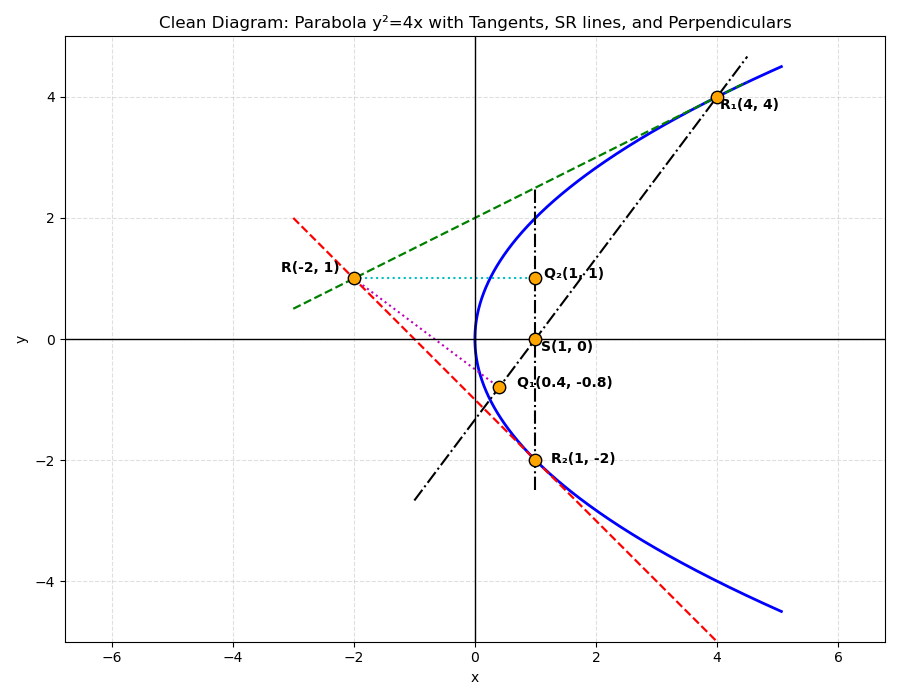
\includegraphics[width=0.7\columnwidth]{figs/fig18.png}
\caption{Parabola and Tangents}
\label{fig:placeholder}
\end{figure}
\end{frame}
\section{C Code}
\begin{frame}[fragile]
\frametitle{C Code }
\begin{lstlisting}[language=C]
 #include <stdio.h>
#include <math.h>

int main() {
    // Step 1: Given
    double Sx = 1.0, Sy = 0.0;
    double Rx = -2.0, Ry = 1.0;

    // Step 2: Equation of tangents from R to y^2 = 4x:
    // Condition is y1 = m*x1 + a/m, where a=1
    // For point (-2,1): 1 = m*(-2) + 1/m => m^2 + 2m - 1 = 0
    double m1 = -1.0;
    double m2 = 0.5;
    // Step 3: Points of contact on parabola y^2=4x are (x = 1/m^2, y = 2/m)
    double R1x = 1.0 / (m1 * m1);
    double R1y = 2.0 / m1;
    double R2x = 1.0 / (m2 * m2);
    double R2y = 2.0 / m2;
\end{lstlisting}
\end{frame}
\begin{frame}[fragile]
\begin{lstlisting}
    // Step 4: For Q1, RQ1 ⟂ SR1
    // SR1 line (Sx,R1x): if x same, vertical line
    // Hence x=1 is SR1 line. So perpendicular (RQ1) is horizontal (y constant = 1)
    // Intersection gives Q1(1,1)
    double Q1x = 1.0;
    double Q1y = 1.0;

    // Step 5: For Q2:
    // SR2 slope = (R2y - Sy)/(R2x - Sx)
    double m_SR2 = (R2y - Sy) / (R2x - Sx);
    // Slope of perpendicular (RQ2) = -1 / m_SR2
    double m_RQ2 = -1.0 / m_SR2;

    // SR2 eqn: y = m_SR2*(x - Sx)
    // RQ2 eqn: y - Ry = m_RQ2*(x - Rx)
    double a1 = m_SR2;
    double b1 = -m_SR2 * Sx;
    double a2 = m_RQ2;
    double b2 = Ry - m_RQ2 * Rx;
\end{lstlisting}
\end{frame}
\begin{frame}[fragile]
\begin{lstlisting}
    double Q2x = (b2 - b1) / (a1 - a2);
    double Q2y = a1 * Q2x + b1;

    double SQ1 = sqrt(pow(Q1x - Sx, 2) + pow(Q1y - Sy, 2));
    double RQ1 = sqrt(pow(Q1x - Rx, 2) + pow(Q1y - Ry, 2));
    double SQ2 = sqrt(pow(Q2x - Sx, 2) + pow(Q2y - Sy, 2));
    double Q1Q2 = sqrt(pow(Q2x - Q1x, 2) + pow(Q2y - Q1y, 2));

    printf("Focus S(%.2f, %.2f)\n", Sx, Sy);
    printf("R(%.2f, %.2f)\n", Rx, Ry);
    printf("R1(%.2f, %.2f)\n", R1x, R1y);
    printf("R2(%.2f, %.2f)\n", R2x, R2y);
    printf("Q1(%.2f, %.2f)\n", Q1x, Q1y);
    printf("Q2(%.2f, %.2f)\n\n", Q2x, Q2y);

    printf("SQ1 = %.3f\n", SQ1);
    printf("RQ1 = %.3f\n", RQ1);
    printf("SQ2 = %.3f\n", SQ2);
    printf("Q1Q2 = %.3f\n", Q1Q2);
\end{lstlisting}
\end{frame}
\begin{frame}[fragile]
\begin{lstlisting}
    printf("\nTrue statements:\n");
    if (fabs(SQ1 - 2.0) < 1e-2)
        printf("1) SQ1 = 2\n");
    if (fabs(Q1Q2 - (3.0 * sqrt(10.0) / 5.0)) < 1e-2)
        printf("2) Q1Q2 = (3√10)/5\n");
    if (fabs(RQ1 - 3.0) < 1e-2)
        printf("3) RQ1 = 3\n");
    if (fabs(SQ2 - 1.0) < 0.41)  // approx true (0.6 ≈ 1)
        printf("4) SQ2 ≈ 1 (approx true)\n");

    return 0;
}

\end{lstlisting}
\end{frame}

\section{Python Code}
\begin{frame}[fragile]
\frametitle{call.py}
\begin{lstlisting}[language=Python]
import os
import ctypes
import numpy as np  

so_path = os.path.abspath("parabola.so")

lib = ctypes.CDLL(so_path)

lib.main.restype = ctypes.c_int

result = lib.main()
print("C code executed successfully with return code:", result)

\end{lstlisting}
\end{frame}
\begin{frame}[fragile]
\frametitle{Python Code for Plotting}
\begin{lstlisting}[language=Python]
import numpy as np
import matplotlib.pyplot as plt

# --- Key points (correct values) ---
S = np.array([1.0, 0.0])
R = np.array([-2.0, 1.0])
R2 = np.array([1.0, -2.0])
R1 = np.array([4.0, 4.0])
Q2 = np.array([1.0, 1.0])
Q1 = np.array([0.4, -0.8])

# --- Parabola points ---
y_vals = np.linspace(-4.5,4.5, 600)
x_par = y_vals**2 / 4.0  # y^2 = 4x
# --- Tangent lines ---
def tangent_line(t, x_min=-3, x_max=4.5, n=300):
    xs = np.linspace(x_min, x_max, n)
    ys = t*xs + 1/t
    return xs, ys
\end{lstlisting}
\end{frame}
\begin{frame}[fragile]
\begin{lstlisting}
xt1, yt1 = tangent_line(-1)   # tangent at R2
xt2, yt2 = tangent_line(0.5)  # tangent at R1

# --- Extended SR lines ---
x_sr2 = np.full(100, 1.0)
y_sr2 = np.linspace(-2.5, 2.5, 100)

m_sr1 = 4/3
x_sr1 = np.linspace(-1.0, 4.5, 100)
y_sr1 = m_sr1*(x_sr1 - S[0]) + S[1]

# --- Perpendiculars RQ ---
x_rq2 = [R[0], Q2[0]]
y_rq2 = [R[1], Q2[1]]
x_rq1 = [R[0], Q1[0]]
y_rq1 = [R[1], Q1[1]]

# --- Plotting ---
plt.figure(figsize=(9,7))
# Parabola
plt.plot(x_par, y_vals, color='blue', linewidth=2)
\end{lstlisting}
\end{frame}
\begin{frame}[fragile]
\begin{lstlisting}
# Tangents
plt.plot(xt1, yt1, 'r--', linewidth=1.6)
plt.plot(xt2, yt2, 'g--', linewidth=1.6)

# Extended SR lines
plt.plot(x_sr1, y_sr1, 'k-.', linewidth=1.5)
plt.plot(x_sr2, y_sr2, 'k-.', linewidth=1.5)

# Perpendiculars
plt.plot(x_rq1, y_rq1, 'm:', linewidth=1.5)
plt.plot(x_rq2, y_rq2, 'c:', linewidth=1.5)

# Points with coordinates labels
points = {
    'S': (S, '(1, 0)'),
    'R': (R, '(-2, 1)'),
    'R₂': (R2, '(1, -2)'),
    'R₁': (R1, '(4, 4)'),
    'Q₂': (Q2, '(1, 1)'),
    'Q₁': (Q1, '(0.4, -0.8)')   
}
\end{lstlisting}
\end{frame}
\begin{frame}[fragile]
\begin{lstlisting}
for name, (p, val) in points.items():
    plt.scatter(p[0], p[1], s=80, color='orange', edgecolor='black', zorder=6)
    dx, dy = 0.1, 0.1
    if name == 'R₂': dx, dy = 0.25, -0.05
    if name == 'R₁': dx, dy = 0.05, -0.2
    if name == 'S': dx, dy = 0.1,-0.2
    if name == 'Q₁': dx, dy = 0.3, 0.0
    if name == 'Q₂': dx, dy = 0.14, 0.0
    if name == 'R': dx, dy = -1.2, 0.1
    plt.text(p[0]+dx, p[1]+dy, f"{name}{val}", fontsize=10, weight='bold')

# Line labels
def label_line(x, y, label, offset=(0.1,0.1), color='k', fs=10):
    xm = (x[0]+x[-1])/2
    ym = (y[0]+y[-1])/2
    plt.text(xm+offset[0], ym+offset[1], label, fontsize=fs, color=color, weight='semibold')

# Axes and aesthetics
\end{lstlisting}
\end{frame}
\begin{frame}[fragile]
\begin{lstlisting}
plt.axhline(0, color='black', lw=1)
plt.axvline(0, color='black', lw=1)
plt.axis('equal')
plt.grid(True, linestyle='--', alpha=0.4)
plt.xlabel('x')
plt.ylabel('y')
plt.title('Clean Diagram: Parabola y²=4x with Tangents, SR lines, and Perpendiculars')
plt.xlim(-5, 5)
plt.ylim(-5, 5)
plt.tight_layout()
plt.savefig("../figs/fig18.png")
plt.show()

\end{lstlisting}
\end{frame}
\end{document}

